\documentclass[10pt,a4paper,twoside,twocolumn]{article}

\usepackage[T1]{fontenc}
\usepackage[utf8]{inputenc}
\usepackage{lmodern}

\usepackage{gwa}
\usepackage{graphicx}
\usepackage{url}

\usepackage{listings} 
\usepackage{stfloats}

\newcommand{\eg}{e.\,g., }
\newcommand{\ie}{i.\,e., }
\def\lqq{\lq\lq}
\def\rqq{\rq\rq}
\def\dq#1{\lqq #1\rqq}
\def\zitat#1{\lqq \emph{#1}\rqq}

\begin{document}

\title{Distributed Version Control with Git}

\author{
  \authN{Richard Plangger, Simon Zünd and Klaus Nigsch}\\
  \matNr{1025637, 1025990, 1025991} \\
%  \kennZ{182, 182, 182}\\
  \authI{Institute of Computer Engineering}\\
  \authU{Vienna University of Technology}\\
  \email{e\{1025637,1025990,1025991\}@student.tuwien.ac.at}
}

\maketitle

% abstract
\abstract {
Distributed Version Control systems enable people to work on the same project, at the same time in different locations. We will not only describe how and why they are used, but also compare the most popular Distributed Version Control Systems against each other and show how they differ from centralized systems. The second part of the paper will describe Git, a system developed by Linus Torvalds to handle the source code of the linux kernel. We will explain the most important commands and give some technical background information. This paper will clarify, why Distributed Version Control Systems became so popular and what advantages they can bring into a programmer's daily work.
}

% - Introduction
\section {Introduction}

Managing a project of software development is not a simple task. Depending of the size of the project, a few or even a whole bunch of people are involved in the development. This fact creates a few problems. For instance when several people work at one source file, or files are getting outdated, because someone else has modified it already. Problems like these are still very common in software development and sooner or later a good solution has to be found to minimize these problems or you will lose control. One might ask how the best way of handling these problems looks like.
This is exactly what this work is about. It is about Version Control Systems, actually Distributed Version Control Systems. "`Distributed"' ones are the modern approach of Version Control Systems, compared to the "`Centralized"' models. However, this work does not only explain these Distributed Version Control Systems in general, it also provides a deeper look into one of these systems, named Git.
Git was chosen because it is currently our favourite Distributed Version Control System out of all of them. For us, it was clear from the beginning that we use Git to handle the writing progress of this scientific paper you are currently reading. This shows that we are really into Git and did not simply chose a random system out of the pool of modern Distributed Version Control Systems..
By reading this paper, you will get an insight look into the world of Distributed Version Control Systems, how and why they work.

Section \ref{whyrevisioncontrol} explains why Revision Control is needed at all. Section \ref{dvcshistory} provides a brief history of Distributed Version Control Systems (DVCS). Section \ref{explanationofterms} presents the basic terms used in DVCS showing how DVCS actually work. Section \ref{changeofworkflows} shows in what way the workflows changed with the change from the centralized systems to the distributed ones. Section \ref{critismondvcs} presents a critical view on the DVCS world, mentioning possible problems in the DVCS model. Section \ref{githistory} introduces Git beginning with a short history. Section \ref{howdoesgitwork} focusses on Git and provides a deeper look into Git and what Git does internally. Section \ref{comparisontootherdvcs} compares Git to other common DVCS statistically. Section \ref{currentdevelopment} presents what the current development around the whole DVCS topic looks like, pointing out a few popular and rising projects. Section \ref{conclusion} finally gives a short conclusion. The paper ends with the references used. 


\section{Why revision control}

\zitat{Revision control is the process of managing multiple versions of a piece of information.}
\cite[Chapter 1]{hgbook2009}

Many people are not aware of the fact that they do revision control in their daily work. For example they make a document or write a program and send it via E-Mail to another person. This person may change the document and send it back. Or when someone is working on a document. Every time he saves it he may give the document a new name with a incrementing number so that he has a history of his work.

All this kind of work can be referred to as revision control. It helps people to keep track of what they have done.

In the history of computer science many systems were designed and implemented which automated this process of revision control. Some of them turned out to work very well, others did not.

Advantages of using a Revision Control System:
\begin{itemize}
\item People have the possibility to work on the same project at the same time. They even can work on the same file simultaneously. The RCS will handle conflicts if some may occur.
\item If bugs or errors were introduced, it is possible to revert the project to a previous version or stage.
\item The system will keep track of each step the project takes. It will log who has made changes, how these changes look like and when they were made.
\end{itemize}

As seen above, using such a system may help organizing project different sizes.


% -
\section {A brief history of Distributed Version Control Systems}

Before Distributed Version Control Systems (DVCS) were introduced, Centralized Version Control Systems (CVCS) were the common system to handle team development.
These traditional CVCS were built up in the following way: One central server stores the content of the project, along with a history of the changes made. This means that the complete content (all changes) have to pass the central server. In other words: One developer commits changes (to the server), and all other developers have to update to this version from the server.

//INCLUDE PICTURE - CENTRALIZED VCS

Although this system might look simple and effective at the first place, it has quite a few drawbacks.


\cite{branchingstrategies2010}

% - General description DCVS (Properties)
		
		
		
% - A brief history of DCVS (Klaus)

% - Begriffserklärung (Simon)
\section{Explanation of terms}

In this section we want to explain some of the phrases, words and terms used through out the article so the 
readers unfamiliar with version control might get an overall idea what version control is about.

We will often refer to CVS\footnote{http://www.nongnu.org/cvs/} (Concurrent Versions System) and SVN\footnote{http://subversion.apache.org/} (Subversion) which are the most used centralized Version Control Systems.

It is also noteworthy that the term “Revision Control System (RCS)” may be used instead of “Version Control System (VCS)”. These two are interchangeable. In other books and articles revision control may also be referred to as “Software Configuration Management (SCM)” or “Source code control”. Those terms have different meanings in different contexts and there is an ongoing discussion about the definitions of those terms.

\subsection{Repository}

A repository in DCVS terms is a folder which can contain sub folders and files of all categories. 
This folder is tracked by the DCVS so there is a history for every file whether it was renamed, deleted or changed. 
How these changes are tracked is different from system to system. CVS for example “isolates” 
files and handles them individually. So each file has its own version number. If you change a file, CVS will 
save the delta (i.e. what has changed) and give the file a new number. SVN does it a little bit 
different. If you change one file, the whole repository gets a new version number, usually count from 1, 2 to n. 
In SVN terms such a version of the repository is referred to as a “revision”.

Git also handles the repository as a whole. It saves each new file version as a whole and not just the delta as SVN and CVS does. 
In Git there are no incrementing version numbers, instead git uses the SHA-1 checksum. For each file there is such a 
checksum and the checksum which represents a certain revision is a sum of these checksums. 
This explanation might not be 100 percent correct but its a good approximation for those unfamiliar with version control.


\subsection{Commit}

Committing means that you make all your changes you have made to some files inside the repository permanent. 
After committing you have a new revision of your repository. Its possible to move back and forth between commits so you can work 
from an older version if you have screwed something up.

Normally with each commit there is saved some meta information like, who has committed and what has been done since the last commit. 
It's good practice to give detailed information about what files have changed and the purpose of these changes, so others working 
on the repository know whats going on.


\subsection{Checkout}

In CVS and SVN a checkout is the operation of creating a local working copy of a certain version from the 
central repository. In git checkout has a slightly different meaning. Creating a local working copy in git is 
called “clone”. Checkout is called the operation of switching between different versions and branches. I.e. 
you change your local working copy to another version.


\subsection{Branch}

Branching means that you diverge from your main line and continue working without messing up the main line of 
development. Branches are a feature where Git really shines because they are very lightweight and really fast compared to other VCSs.

\begin{figure}[ht]
  \centering
  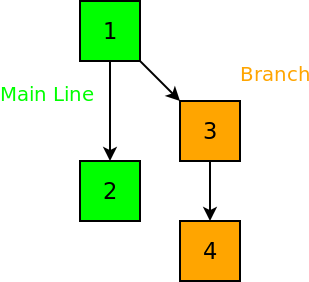
\includegraphics[width=0.4\textwidth]{img/Gen_Branch}
  \caption{Basic branching}
  \label{fig:gen_branch} 
\end{figure}

Figure \ref{fig:gen_branch} shows a little example how such a branch looks like. The green version 1 in 
this example is the initial commit with some files. Now developer A continues development in the main line by fixing 
some bugs and improving the current version. Developer B know wants to add some new experimental 
features to version 1. Because developer B doesn't want to mess up the hopefully stable main line and the 
changes of developer A, he creates a branch where he can develop the new features until they are stable. 
So the orange versions 3 and 4 are the branch and the green versions is the stable main line.


\subsection{Merge}

Merging is called the process of integrating changes to a file which was modified by two people individually 
at the same time. When there are no conflicts the merge can be done automatically, else, a person must resolve 
the conflict. A conflict can occur when both people change the same lines inside a file, so the person who 
merges the changes must decide which version to use or how to integrate both versions into the file.

“Merging branches” does mean that changes made to a branch will be merged into another branch. 
To successfully merging branches they must have a common parent in their history.

\begin{figure}[ht]
  \centering
  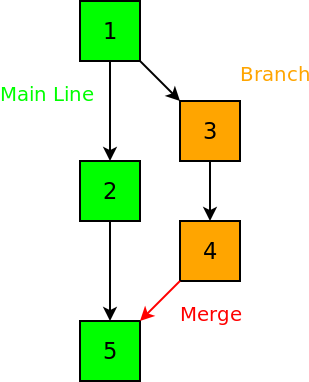
\includegraphics[width=0.4\textwidth]{img/Gen_Merge}
  \caption{Basic merging}
  \label{fig:gen_merge} 
\end{figure}

Figure \ref{fig:gen_merge} shows a later stage of the example from above. The developers decide that 
the new features in version 4 are stable and can be merged into the main line.


\subsection{Tagging}

Tagging means that you mark a certain version or revision with a tag. 
Assigning a tag to a version is just for convenience, normally its used to tag important project milestones. 
For example if your application which you are developing reaches version 1.5, you will assign a tag named “v1.5” 
to the commit or revision which was used to build the “application 1.5” or which represents the “application 1.5”. 
So it will be very easy to find the commit you need in the future if you want an older version of your application.

\begin{figure}[ht]
  \centering
  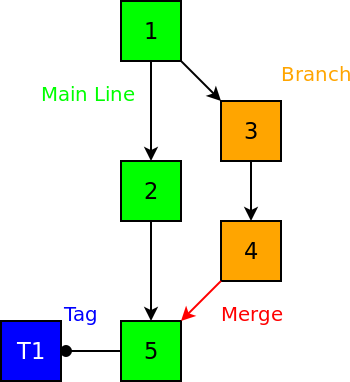
\includegraphics[width=0.4\textwidth]{img/Gen_Tag}
  \caption{Basic tagging}
  \label{fig:gen_tag}
\end{figure}

Figure \ref{fig:gen_tag} shows how the new version 5 from above is tagged with a tag T1.


%	- Changing of Workflows (Simon)
\section{Changing of workflows} \label{changeofworkflows}

With the evolution form Centralized Version Control System to Distributed Version Control Systems there also 
evolved new ways of how development processes can be organized. In this section we show differences 
between centralized and distributed systems, especially how we work with them, where problems can occur by using 
centralized systems and how the distributed systems try to solve them. At the the end of the section we want 
to show some common models to handle projects of different sizes.

\subsection{Workflow differences}

The difference which has the most impact on how we work with the systems is the centralized/distributed aspect. 
A distributed system saves the whole project history locally, also all operations are performed on the local clone. 
This is a huge advantage over centralized systems. A developer has to be connected to the central 
repository to work on a project. However, the developer can work on his project, but 
he can not work with the version control system. So the distributed systems have a “mobile” advantage. 
Developers can work on their projects wherever they are and there is no need for a connection with the 
Internet or the company network.

It is not only about the remote connection, it is also about the server availability. If the server, where 
all the repositories are hosted, goes offline for whatever reason, all developers are cut off from development.

Because centralized systems have to talk with their servers for many operations they do not work as fast as 
a distributed system does. It takes a lot more time to checkout a previous version over the network 
then reverting back to a previous version locally. This fact has an impact on how developers use the system. 
If operations are very fast and take only little time developers may use them more often. They may commit 
more often not only because it is fast, but because their commit can not break the whole project. 
In centralized environments every developer \emph{must} only commit code which is stable so the project 
itself stays in a stable state. The implication of this need for stable commits is that developers won't 
commit for a longer time so their code base diverges more from the main line and it is very hard 
to merge the changes back to the main line.

The next big difference is the aspect of branching and merging. It is not so common to use branches 
in centralized systems than it is in distributed ones. SVN for example doest not have a separate branch 
mechanism at all. \cite[Apache\_Subversion\#Tag- und Branchkonzept]{wikipedia}
It is the task of the SVN administrator to organize the main line, branches and tags on the server. 
So it is very hard to create a branch just to implement some new feature or to fix a single bug. Another 
point is that all the branches are visible and accessible for everyone. So there can only 
be one branch called “test”.

As the reader may see in the section about Git, it is very common in distributed environments to 
do a lot of branching and merging. The reason for this is that DVCS like Mercurial, Git and Baazar 
have the design goal to make branching and merging easy and fast. So a developer may create a branch 
for each issue in the issue tracker. When he has solved the issue he merges the fix back to the main 
line and he can delete the branch. That is also true for new or experimental features or just for some sort 
of testing purpose. Nobody will ever know that there was a branch except the developer publishes 
it and allows other developers to pull his branch into their local repository. If they do so, it 
does not mean that they have to merge the branch or use it at all. If someone deletes
the branch locally, nobody else will ever recognize it.


\subsection{Distributed workflow models}

These models were described in the Pro Git Book \cite[chapter 5.1]{gitpro2009} and are 
worth mentioned here. The images are also adopted from the book but made a little bit smaller and more compact.

In a distributed environment every developer acts as a contributor and as a server at the same time. So there are more 
possibilities to organize development processes than there are in a centralized environment.


\subsubsection{Centralized Model}

\begin{figure}[ht]
  \centering
  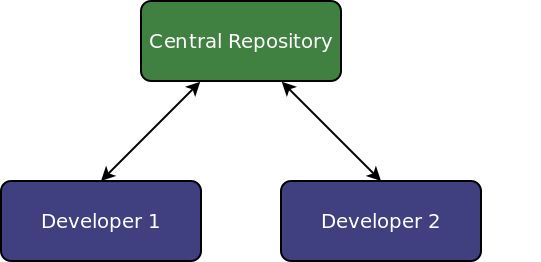
\includegraphics[width=0.5\textwidth]{img/Mod_Central}
  \caption{Centralized Model}
  \label{fig:mod_centralized} 
\end{figure}

First of all a DVCS can be used like a normal centralized system (see Figure \ref{fig:mod_centralized}). One developers repository or a extra repository acts as the central hub. Before a developer can push his work to the central repository he has to merge all the changes done to the central repository into his local repository. This model works well for small project teams as well as for people used to centralized systems and are not familiar with distributed workflows.


\subsubsection{Integration-Manager Workflow}

\begin{figure*}[tbp]
  \centering
  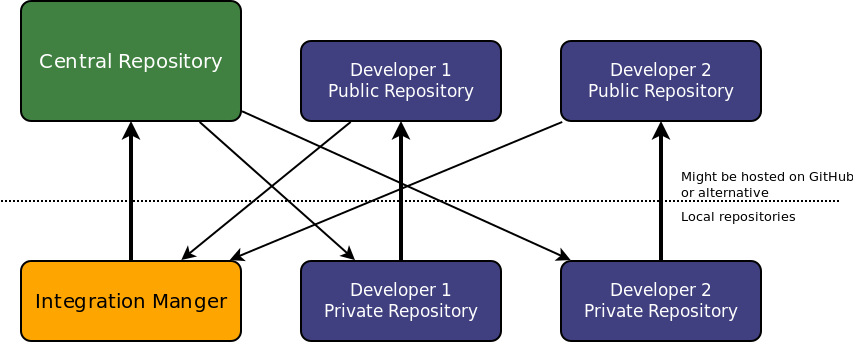
\includegraphics[width=\textwidth]{img/Mod_IntegrationManager}
  \caption{Model with an Integration Manager}
  \label{fig:mod_intMan} 
\end{figure*}

This workflow became very common as services like GitHub started to evolve. In
this model (see Figure \ref{fig:mod_intMan}) just a handful of people has write access to the central (or “official”) repository. 
These people are called integration managers. In smaller projects there might be just one integration manager and their 
number may grow with the project size. The task of an integration manager is to pull changes from developers and merge 
them into the central repository. They also have to decide which changes are worth merging.

Every developer has also a public repository, so the integration managers and the other developers can easily pull from 
each other. The real work is done in the private local repositories of the developers. Once changes are merged into the 
official repository the developers have to merge them back into their private repositories, so they have the same state as the official one.

This model works very well in open source projects, because it is possible to host OSS (Open Source Software) on 
sites like GitHub for free, so the public repositories of the developers and the integration managers might be hosted there.


\subsubsection{Dictator and Lieutenants Workflow}

\begin{figure}[ht]
  \centering
  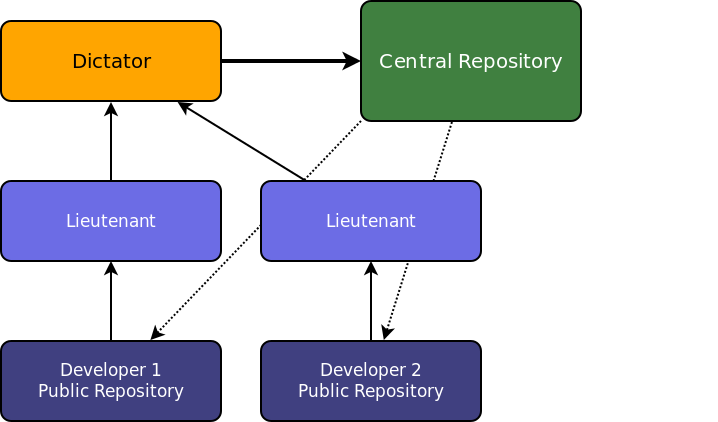
\includegraphics[width=0.5\textwidth]{img/Mod_Dictator}
  \caption{Dictator and Lieutenants Model}
  \label{fig:mod_dictator} 
\end{figure}

This workflow is an enhancement of the “Integration-Manager Workflow”. Instead of having a handful of 
integration managers which are all responsible for the whole code base, there is a hierarchy of integration 
managers which are responsible for a certain module or subsystem. The topmost integration manager is called 
the “dictator”, and the integration managers on the levels below are called “lieutenants”.

The advantage of this model is that the dictator or a lieutenant does not have to check every change from 
each developer, instead he can just trust the lieutenants below him and pull changes from them. This model 
is not very common because it is very hierarchical and only starts to become effective once a project gets really big and complex.

An example is the Linux kernel, where Linus Torvalds acts as the dictator and the lieutenants are 
responsible for the different subsystems of the kernel. \footnote{http://en.wikipedia.org/wiki/Linux\_kernel\#Maintenance}


%	- Critism on Distributed Version Control Systems (Klaus)
\section{Critism on Distributed Version Control Systems}\label{critismondvcs}

Despite all the advantages Distributed Version Control Systems provide, there is also heavy critism going on. Hyrum Wright, president of the Subversion Corporation clearly states a downside of DVCS: 

\textit{"`In my experience, when a team moves to a Distributed Version Control Tool, they are not really doing that for workflow purposes. Their workflows remain the same. They are doing it because they appreciate the tooling, the features that are available in those tools for use in their team. They still usually have a centralized location where the code lives, very much like a central Subversion repository."'} \cite{subversionandgit}

Hyrum Wright confronts the DVCS community with an argument that is justified. A large number of DVCS projects additionally use a Subversion repository just to store a main version of the product, a version representing the reference point. This is a definite indicator to what Hyrum Wright stated - people are just using DVCS for the features available in DVCS tools, not because they appreciate the workflow. It is also very common in distributed workflows to have a central repository, not a SVN one but a distributed repository that is declared as the central or "blessed" repository as called in the Pro Git Book \cite[Chapter 5.1]{gitpro2009}. This point is justified comparing the workflows described in the previous section. Every workflow mentioned there has such a central reference point.

Hyrum Wright goes even further as he states that Subversion learned from DVCS and will soon provide features in SVN so far just available in DVCS. \cite{subversionandgit} The goal that SVN is trying to reach is obvious: If Subversion has no disadvantages tool-wise and the workflows are anyways less decisive for people, the SVN community will grow dramatically.

Another critism is directly confronting the DVCS workflow. In opposite to the DVCS community, the CVCS community states that the DVCS workflows are not only confusing, but also a big problem. Their statement says that any growing DVCS project will sooner or later have problems creating a final version. Every user has different branches and outdated versions of the project. At some point of time, the team loses control over the content and they are not able to merge a final version, because there is no real reference point anymore. 




% GIT
  %   +-- History
  \section {A brief history of Git}\label{githistory}

The Linux kernel development was originally handled by a patch-emailing system, but in 2002 Linus Torvalds and his development team moved to the Source Code Management (SCM) system BitKeeper. BitKeeper was a commercial product free to use for open-source projects, however, Linus Torvalds decided to make use of it. Although Linus Torvalds' philosophy concering software is "`Open Source is the only way to make software"' \cite{googletechtalk2007}, he uses the best software available for his needs, commercial or not.
In 2005, BitMover (developer of BitKeeper) stopped their support for open-source projects. That's why soon after Linus was desperately trying to find a new system to handle the Linux kernel development, without success. They were either slow or simply not distributed. For Linus it was essential that the SCM system is distributed and has a high performance. If a system didn't provide only one of these aspects, the SCM system simply wasn't of any use for him. When Linus did not find any SCM system he could use, he simply decided that it is best to write his own SCM - Git - which he already released in April 2005. Linus Torvalds commented his decision to write Git in the following way: "`I decided that I can write something better than anything out there in two weeks. And I was right!"'\cite{googletechtalk2007}

In the Git development, design ideas were based on what developers learned from BitKeeper. Although Git was BitKeeper oriented, it became a completely new software with numerous advantages, including:

\begin{itemize}
	\item incredible speed
	\item high efficiency, especially in large projects
	\item outstanding branching system
\end{itemize}
\cite{gitpro2009}

Git became a huge success. Originally used for nothing but the Linux kernel, soon other projects moved to Git to handle their development. A few popular examples are X.org, Fedora, Samba and Ruby on Rails. \cite{gitinternals2008}
  %   +-- How does git work
  \section{How does git work internally?}\label{howdoesgitwork}

To understand how git works we need to know some basic commands.

\subsection {Basic local commands}

As any other VCS git stores its data in the repository directory.
There are two major ways to get a repository.
One would be by simply creating a new empty git repository in your directory of choice:
\begin{lstlisting}
$ git init
\end{lstlisting}
This command creates a new subdirectory .git/ where all your version control
data is stored. \cite[Page 55]{gitinternals2008} \\
The second is to clone an existing repository over an URL. Possible protocols
are FILE SSH HTTPS HTTP or GIT. Of course on the target location must host a
git repository:
\begin{lstlisting}
$ git clone 
    git://github.com/rails/rails.git
\end{lstlisting}
Git will clone the whole ruby on rails project from github and we're
ready to get to work. \cite[Page 56]{gitinternals2008} \\

After we have a new repository we can add some content:
\begin{lstlisting}
$ touch README
$ git status
$ git add README
$ git commit -m "Added README file"
\end{lstlisting}

This code produces an empty README file. The status command displays any change
of the repository. There we can see that the README file has been added and we
track this file simply by telling git to add the file to the index. Additionally
git now stages the file, but we are going to cover the staging feature later in the next
section. Then we commit the changes with a short and descriptive message. After
this git stores the changes into the repository and points the default master
branch to the new commit. \cite[Page 55]{gitinternals2008} \\

\subsection {History}

With every commit Git will append information to the history of your project. This history
can be browsed using the \emph {git log} command:

\begin{lstlisting}
$ git log
commit 8133a...
Author: User <user@provider.org>
Date:   Wed Nov 17 19:29:03 2010 +0100

    [commit message]
    
commit 3131f...
Author: User <user@provider.org>
Date:   Wed Nov 17 19:29:03 2010 +0100

    [commit message]
    
...
\end{lstlisting}

Each commit consists of 4 parts: the commit SHA1 string, the author with his e-mail address, the commit date and a short descriptive message.
But this is not all you can see in the history. With several additional commands you can format the history or even display all the changes.
As an example this code formats the history quite different:

\begin{lstlisting}
$ git log 
   --pretty=format:"%h, %ar : %s"
8133ae1 4 days ago : fix issue 8645
741a1bc 4 days ago : merged crazyidea
3131fd0 4 days ago : added scripts
\end{lstlisting}

There are several more formating place holders that can be used. \cite[Chapter 2.4]{gitpro2009} \\

As an example for the capability of the log command, there is a shell script\footnote{https://github.com/d1rk/git-ftp on 21.11.2010} on GitHub that allows you to upload your git repository over the ftp protocol. This script uses the git log command to get enough information to upload the changes to the ftp-server. 

\subsection{Git over network}

After there has been committed a huge amount of work in the local ruby on rails
repository we can share the work telling git:

\begin{lstlisting}
$ git push origin master 
\end{lstlisting}

This command will only succeed if you have the appropriate access rights to the
project. But if we had them, the master parameter tells git to take the default
branch and transmit the changes to the host. We could also specify any other
branch and transmit it to the destination host. \\ 

Also one should know that the origin parameter is our destination. You can
simply add many different socalled remotes:

\begin{lstlisting}
$ git remote add [name] [url]
\end{lstlisting}

This command links a short name to any url and you can share your
work over any network git is designed for. \cite[Chapter 2.9]{gitpro2009}  \\

The last very important command is:
\begin{lstlisting}
$ git fetch origin
\end{lstlisting}

The fetch command is used to get work from other people of your project since
the last time you fetched. Very important is that this command does not
automatically merge the new updates into your local master branch. It just
downloads the updates and creates a new brach FETCH\_HEAD. Then you have to
manually merge the branch FETCH\_HEAD to the desired branch. 
If you dont need this very powerful feature you can simply execute:
\begin{lstlisting}
$ git pull origin
\end{lstlisting}
Git will automatically merge the changes into your master branch.
\cite[Chapter 2.9]{gitpro2009} \\

\subsection {Staging}

Now that we convered the fundamental basics of git. We can take a deeper look at
some parts of the logic used by git. One high level feature of git is the
\emph{interactive adding}. We create a new repository and add a file and commit
it. If we modify the same file again and try to commit with the command above,
git will not apply the modified file to the repository. This is because this file is
not explicitly added to the socalled staging mode. You have to explicitly add
the modified file to the staging mode and commit. This feature gives you much
more control over what goes into your repository or not. This feature is often
ignored and you can simply commit a unstaged file with this command:

\begin{lstlisting}
$ git commit -a -m "message"
\end{lstlisting}

The parameter \emph{-a} automatically adds the file to the staging mode and
commits it. \cite[Chapter 2.2]{gitpro2009}

The picture\footnote{http://progit.org/figures/ch2/18333fig0201-tn.png accessed on 
09.11.2010} taken out of the git pro book illustrates how files change their
lifecycle modes:

\begin{figure}[h]
  \centering
  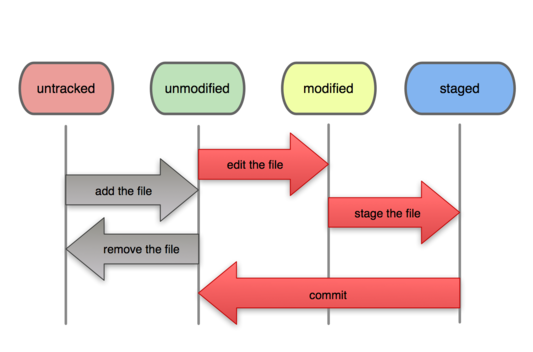
\includegraphics{img/file_status_lifecycle}
  \caption{File status lifecycle}
  \label{fig:File status lifecycle}
  
\end{figure} 

As we can see there are four modes a file can have. First we have to track them
once to get them into the lifecycle. If we modify we can use \emph{-a} on the
commit command to automatically stage and commit them, or we can take alot more
control of our repository and stage them manually and avoid mistakes and
redundant changes that do not belong to a certain commit.
We can simply get information about the mode using the git command
\emph{status}. \cite[Chapter 2.2]{gitpro2009} 

\subsection{How does git store its data?}
Git uses a unique store model compared to other common DVCS like Baazar or Mercurial. 
In tradional distributed or normal version control the system keeps differences between revision A and B. 
These changes are saved and marked with a revision number. 
So you can, at any time, switch back to any revision and rebuild the complete content.
This does have some major downsides which we will see later. \\
Git does handle it quite different. It takes socalled \emph{snapshots} in every
new version. So if file A changes in your repository the next commit git will take a new snapshot of this file and all other files. 
To reduce overhead not changed files are linked to the identical file in the previous verion. 
It creates a new minifile system rather than a VCS, enabling you all the features normal version 
control would give you and gives you some additional on top of it. \cite{gitpro2009} 

\subsection{Checksums for integrity}

\zitat{ Every single piece of data, when git tracks your content, we compress it
we delta it against everything else, but we also do a SHA1 hash of the content
and we actually check it when we use it. If you have discorruption if you have
dramcorruption if you have any kind problems at all git will notice them. It is
not a question of if, it is a guarantee } \cite{googletechtalk2007}

Git is secure. As you can see in Linus Torvalds speech, git uses the SHA1-Hash
as an integrity feature. Secure Hash Algorithm 1 is a string with 40 hexadezimal
characters. It creates a checksum of two pieces of data and makes it nearly
impossible that 2 files have the same checksum. This makes discorruption or loss
of data impossible without notice. \cite[Chapter 1.3]{gitpro2009}

\subsection {Branching}

Branching is a major features in git. But also like the staging mode
branching can be skipped and you can just stick to the master
branch. \\
Assumed we have a new feature request for the ruby on rails project called
newfeature we add a branch:
\begin{lstlisting}
$ git branch newfeature
$ git checkout newfeature
\end{lstlisting}

To understand what branching do technically we have to take a deeper look at
what a commit does internally: \
After you execute the commit command Git creates a new commit object that
contains a pointer to the snapshot of your content you staged, some metadata and
pointers to you previous commits. If there are zero previous commits no pointer
is stored and if you merged a branch the commit can point to multible previous commits.

After staging a single file, Git creates a checksum and stores the version in the repository. Additionally it adds the
checksum to the staging area. This file is now a blob object.
When you execute the commit command, Git will create checksums for each
subdirectory and adds this tree object to the repository. Finally git creates
the commit object that contains the metadata and a pointer to the root object
tree. This is necessary to be able to recreate the snapshot.

We have three new objects in our repository describing the part of the history
of the project. There is one blob for the file we staged, the tree object that
points to the blob and a commit object that points to that tree object including
all metadata, like commit message and author. 
\\

Lets see what the releationship between these objects look like:

\begin{figure}[h]
  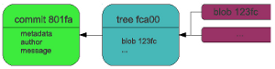
\includegraphics{img/branch2}
  \caption{Git objects after a commit}
  \label{fig: git objects after a commit}
  %\author{Richard Plangger}
\end{figure}

It is obvious that very commit looks like this and every commit, exept the first
has one or more parents.
A branch is just a moveable pointer towards a commit. Also the master branch is
one of those ligthweight pointers towards a commit. In addition there is a
pointer called HEAD which specifies which branch we are currently on. So by
executing the command \emph{git checkout [branchname]} we move the HEAD
pointer. 

Now it is time to make a new commit in the crazyidea branch and switch back to
the master branch and also commit some changes.
This could look like this:
\begin{figure}[h]
  \centering
  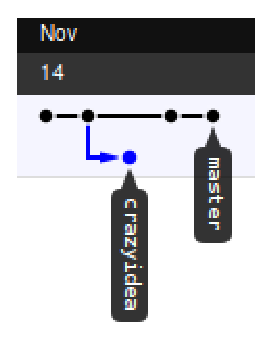
\includegraphics{img/branch3}
  \caption{The new branch crazyidea}
  \label{fig: a new branch}
\end{figure}

There has been created a new commit pointing to one commit of the master branch.
The new commit in its own branch now contains the history from the master branch
to the commit where it was splitted from and the changes in the new
branch. The last two commits that has been made in the masterbranch are not
visible in our new branch. 

Because a new branch in git is equal to a single
file with the SHA1 checksum branches are very cheap. In other version control systems branching means to
fully copy the whole content into a new folder and not just create a 41 byte
file. This can take seconds or even minutes and discourages developers to use
this powerful feature. \cite[Chapter 3.1]{gitpro2009}

\subsection {Merging}

Merging is the need of putting together data from different branches. Maybe one
day our crazy idea will turn out to be brilliant and also the crazyidea is
stable enough to put it to our master branch we need a way to put them together.
At this point the merge command pops in:

\begin{lstlisting}
$ git merge [branchname]
\end{lstlisting}

Git now merges all differences into the branch we're currently on and we can see
the result:
\begin{figure}[h]
  \centering 
  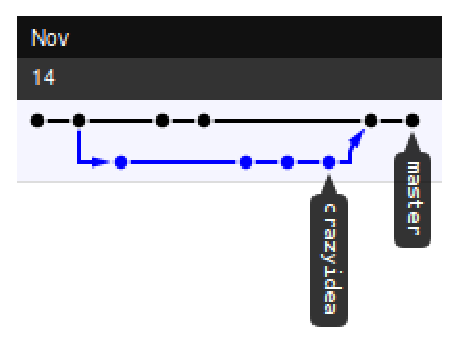
\includegraphics{img/merge1}
  \caption{Merged the crazy idea into the master branch}
  \label{}
\end{figure}

After the merge all data that is not contained in master but in crazyidea is put
together and will be part of master. As we can see this is very powerful feature
that allows developers to be flexible and work on several different parts of the
project, without breaking the whole project. \cite[Page 30-31]{gitinternals2008}

\subsection {What makes git a DVCS?}

Linus Torvalds did a quite good job to summarize what distributed means:

\zitat{Being distributed very much means that you do not have one
central location that keeps track of your data, no single place more important
than any other place \ldots } \cite{googletechtalk2007}

Nearly all commands that git offer you are local operations. There is no need to
have any network connection at all to work on your project and track changes
afterwards. Moreover the whole history of your project is contained in your
local repository. Also all contributors of one project have that history if
they pull from you. Hence no repository has more information about the project
than the other.


  %   +-- Comparison to other DVCS
  \section {Comparison to other DVCS}

There are several more distributed version control systems
we are going to explain some differences to git.
Some are:

  \begin{enumerate}
     \item \emph{Bazaar}. Powered by Cannocial. Handles the whole Ubuntu source
     repository at launchpad.net
     \item \emph{Mercurial} An opensource project initiated by Matt Mackall
     \item \emph{Perforce}. Powered by Perforce Software Inc.
     \item \emph{Visual SourceSafe} Powered by Microsoft
  \end{enumerate}
  
We are going to take a closer look at \emph{Baazar} and \emph{Mercurial}
compared to Git.

\subsection {Data storage}

As already mentioned git uses it's unique storage model creating new snapshots
every commit. Mercurial also thinks of its data as a snapshot. The difference
is though, that basically Mercurial also creates deltas from a revsion A to B.
Those deltas are infact the difference between two revsions. When a cumulative
amount of deltas is stored to a file, Mercurial creates a new snapshot of this file. 
\footnote{\cite {hgbook2009}
http://hgbook.red-bean.com/read/behind-the-scenes.html, section Fast retrieval,
accessed on 14.11.2010}
Baazar TODO!!

\subsection {Speed}

Git claims to be a very efficient system. To mesure that there are several
methods. The website \emph{whygitisbetterthanx.com} did a quite good job to
summarize why git does handle things quite fast.

\subsection {Size}


  %   +-- Current Development. How uses git?
  \section{Current Development of Distributed Version Control Systems}\label{currentdevelopment}

This section contains information about projects and initiatives in the field of Distributed Version Control Systems.

\subsection{GitHub (\textit{http://github.com})}
\begin{figure}[h]
  \centering 
  
\includegraphics{img/github}
  \caption{GitHub logo}
  \label{}
\end{figure}
GitHub is a web-based hosting service coded in Ruby on Rails for projects using Git to handle their codebase. This service was launched in February 2008 and counts to-date (November 2010) more than one million hosted projects. GitHub can be used commercially or for free. By using GitHub for free you confirm that everything you host on GitHub is open source.
Getting started with GitHub is not a problem. The platform offers a large help and support service helping you in using GitHub.
Basically, all you have to do after you successfully installed Git on your computer is generating an SSH keypair, set your username and e-mail and create or fork a GitHub repository, and you are ready to work.
The SSH keypair you are generating is important in terms of security. This keypair identifies you. It is SSH encoded and secure, you do not have a plain text password.
Creating a new GitHub projects means you are setting up a completely new repository. Forking one means you create your own fork of an existing repository. This makes it possible to work on your own fork and modify it in whatever ways you like to, when some time has passed you can also update your fork with the original repository. This whole service is possible because of the open source philosophy of GitHub.

After being finished with all these steps, GitHub provides a URL to clone your project. From this point you are able to work with Git as always. Of course, multiple people can join your repository. They usually have read-only access to the project, as long as you grant them other rights.

GitHub offers a lot of nice features. For example there is a feature showing you who of the project members impacted how much source code and when. This is displayed in a graph. There is also a feature showing you when project branches were merged together along with the states of the branches. This is as well displayed in a graph. Also, GitHub offers a RSS system for all kinds of things like new commits, commentaries etc.
\newline
Popular example projects using GitHub are:
\newline
\begin{itemize}
	\item Perl
	\item PHP
	\item Ruby on Rails
	\item jQuery
\end{itemize}

\subsection{Gitorious (\textit{http://gitorious.org})}
\begin{figure}[h]
  \centering 
  
\includegraphics{img/gitorious}
  \caption{Gitorious logo}
  \label{}
\end{figure}
Gitorious is - as well as GitHub a web-based hosting service for projects using Git to handle their codebase. Gitorious was launched in January 2008. So GitHub and Gitorious are competitors, but GitHub is currently (November 2010) leader in the marketplace for hosting services for Git projects.

Since Gitorious is very similar to GitHub, most of the explanation is not needed. It's important to mention that Gitorious is also free, but supporting commercial projects if you with to. Although Gitorious is quite less popular than GitHub, there are still very popular projects hosted on Gitorious.
\newline
Popular example projects using Gitorious are:
\begin{itemize}
	\item Android
	\item openSUSE
	\item Qt
	\item KDevelop
\end{itemize}


\subsection{BitBucket (\textit{http://bitbucket.org})}
\begin{figure}[h]
  \centering 
  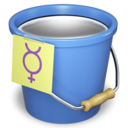
\includegraphics{img/bitbucket}
  \caption{BitBucket logo}
  \label{}
\end{figure}
BitBucket is a free source code web-based hosting service launched in 2008. Compared to other services in that kind, BitBucket hosts and Mercurial and Subversion projects. This service is free for projects containing five or less users included in a project. Projects containing more people cost a monthly fee, ranging up to 80 dollars per month for an unlimited number of users.
\newline
Popular example projects using BitBucket are:

\begin{itemize}
	\item Opera
	\item TortoiseHG
	\item Adium
	\item CodeIgniter
\end{itemize}

\subsection{Launchpad (\textit{https://launchpad.net})}
\begin{figure}[h]
  \centering 
  
\includegraphics{img/launchpad}
  \caption{Launchpad logo}
  \label{}
\end{figure}

Launchpad is a free software collaboration platform launched in January 2004. The Launchpad project supports the idea of free software. Launchpad a web-based hosting service for projects using Bazaar to manage the development. Launchpad, however, is a lot more than just a hosting service. Launchpad offers a whole bunch of services for their users encouraging to develop free software. Aside from code hosting, Launchpad offers a code review section, where users can review your project hosted on Launchpad. Code review gives a public forum where users can rate and discuss the project. Launchpad also offers a But Tracking feature. In open source software, copying software also means you are copying potential bugs. Therefore, Launchpad makes it possible to share bug reports, current statuses and patches and also provides a platform to comment on these.
Another feature of Launchpad is the translations section. Launchpad's philosophy about software and language is that the translators should not be the software engineers. That's why you can allow the Launchpad community to translate your project. Translators are supported by language libraries and suggestions.
Another interesting Launchpad service is the Ubuntu package building and hosting. This service makes it easy to distribute your software to Ubuntu users. You can build and distribute your Ubuntu packages using your personal APT repository.
Specification Tracking is another feature by Launchpad. This offers you to track new features for your software, from the idea to the implementation. This is realized letting the community planning your project and it's road-map. Do not worry: You decide how important a user's idea is and you can also freely ignore them. The last feature of Launchpad is called "`Answers"'. This lets every user build his own knowledgebase. Whenever you come across problems, you can freely add them to your personal FAQ library.

Launchpad is currently (November 2010) hosting more than 20000 projects. Their services are in heavy use, as there are to-date just for example more than 670000 bugs tracked and 1.5 million translations made.
\newline
Popular example projects using Launchpad are:

\begin{itemize}
	\item Ubuntu
	\item Bazaar
	\item MySQL
	\item Inkscape
\end{itemize}

\subsection{Google Code Gerrit \\(\textit{http://code.google.com/p/gerrit})}

Google Code Gerrit is a free online code reviewing system for Git projects by Google. Google users can provide their Git projects and let them be reviewed by other Google users. Gerrit makes use of the Git philosophy: Every user with authority is allowed to commit changes to the Git repository. This way, the project leader does not have to merge all the changes together. Gerrit also has a large discussion group along with a wiki to help new users getting started. 

\subsection{Eclipse with DVCS plugins}

Eclipse, the open source IDE is known for having large plugin support. With the rise of DVCS systems, also DVCS plugins for the popular IDE were developed. Since these plugins (for all the different DVCS) work theoretically the same, just the general use is described here. These plugins add a new bar to Eclipse handling your DVCS project. Inside Eclipse the user will be able to browse through your project including their branches. Also, users are able to perform all the DVCS tasks within Eclipse, thanks to the plugin.
\newline
Popular example DVCS plugins for Eclipse are:

\begin{itemize}
	\item EGit (Git)
	\item Mercurial Eclipse / HGEclipse (Mercurial)
	\item BzrEclipse (Bazaar)
	\item EclipseDarcs (Darcs)
\end{itemize}

\cite{eclipseplugins}

\subsection{Gazest (\textit{http://ygingras.net/gazest})}

Gazest is a community engine based on the Wiki system, started in 2007. Gazest is still not officially launched yet. It is already usable, but not ready for productive use (November 2010). In comparison to other Wikis, Gazest uses a DVCS storage model, heaviely based on the idea of DVCS tools. The idea behind this is, that parallel changes to the Wiki site will be merged just like any DVCS software does. Gazest even encourages users to try out to produce conflicts on a test wiki page to show how good Gazest is in undoing and merging changes parallelly made. Another idea of Gazest is to develop completely new technologies, including branching and merging of multiple Gazest Wiki pages into one single logical unit.


% Conclusion
\section{Conclusion}\label{conclusion}

It can be seen that Distributed Version Control Systems offer a whole bunch of new possibilites for many people to work distributed on one project. Compared to the models of the Centralized Version Control Systems, distributed ones simplify the workflows for every project member, making it possible to work locally and provide or get the work of others as he decides to - or not. Apart from that, Branching in DVCS is a simple yet effective way to implement new features into the project. Effective merging algorithms make it possible for multiple people to work on the same file without having to worry about content loss. \newline
By choosing a modern DVCS like Git, users get a fast and easy-to-learn DVCS which should fulfill all their needs. Community projects like Github connect these users to a large community. Newcomers can not only start their own projects, they can easyiely join an existing project. All these features are making it easy to get started into the DVCS world.

% References
\bibliographystyle{unsrt}
\bibliography{references}

\end{document}
